\chapter{Modeling compositionality}\label{sec:13}

\section{Introduction}\label{sec:13.1}

We have said that one of the most important goals of semantic theory is to understand the compositional nature of meaning, i.e., the knowledge which allows speakers to correctly predict how word meanings will combine in complex expressions. One way of exploring this topic is to construct formal rule systems which model the abilities of speakers in this respect.



Just as syntacticians try to construct rule systems which replicate the judgments of native speakers about the grammaticality of sentences, semanticists try to construct rule systems which replicate the ability of speakers to identify the denotation of an expression in a particular context of use, and in particular, to determine the truth values of sentences in a given context. A crucial step in this kind of analysis is to describe the situation under discussion in very explicit terms, so that predictions about denotations can be easily checked. The explicit description of a situation is called a \textsc{model}, so this general approach to semantics is often referred to as \textsc{Model Theory}.\footnote{A \textsc{model} can also be defined an interpretation under which a given sentence or set of sentences is true \citep{Hodges2013}. But by spelling out the denotations of the basic expressions used in the sentence(s) under discussion, the model also specifies the relevant facts about a particular situation.}



This chapter provides a very brief introduction to the Model Theory approach to the study of compositionality. This approach, which has proven to be remarkably productive, involves stating rules of semantic interpretation for the constituents that are formed by productive syntactic processes. We mentioned two such processes in \chapref{sec:12}: the combination of subject NP with VP, and the combination of modifying adjective with head noun. In this chapter we will provide a bit more detail about how we might formulate the rules of semantic interpretation for these and other constituents.



Our goal in this chapter is not to provide detailed explanation of the Model Theory approach, but merely to give a glimpse of how it works and some sense of what the goals are. This will provide helpful context for our discussion in future chapters of topics such as quantifiers, modality, tense, etc.



\sectref{sec:13.2} provides a brief description of the rationale behind this approach. In \sectref{sec:13.3} we introduce some basic terms and concepts for describing sets and relations between sets, because our rules of interpretation will be stated in terms of set relations. \sectref{sec:13.4} introduces the formal notation that is used for specifying a \textsc{model}, in the sense defined above, and \sectref{sec:13.5} gives some examples of how rules of semantic interpretation might be stated for several types of syntactic constituents. The over-arching goal of all these steps is to account for the ability of native speakers to determine whether the proposition expressed by a given sentence is true or false in some particular context. This, you will recall, has been our benchmark for the analysis of sentence meanings.


\section{Why a “model” might be useful}\label{sec:13.2}

Language is a very complex system. In earlier chapters we have studied a variety of factors that affect how hearers will interpret the meanings of sentences: lexical ambiguity, vagueness, figurative and other coerced senses, implicatures and other pragmatic inferences, knowledge about the world, etc. In order to make progress in understanding how compositionality works, the Model Theory approach attempts to isolate the rules for combining word meanings from these other complicating factors. This same basic strategy is adopted in many other fields of research as well. For example, if medical researchers are investigating genetic factors which may contribute to heart disease or diabetes, they will do everything possible to control for other contributing factors such as diet, age, exercise, life-style, environmental factors, etc. The specification of a test situation in terms of an explicit “model”, as illustrated below, within which the rule system can be tested, is a way of controlling for lexical ambiguity, vagueness, incomplete knowledge about the world, etc.



A model must specify two things: first, the set of all individual entities in the situation; and second, the denotations of the basic vocabulary items of the language, at least those that occur in the expressions being analyzed. This would include words which function as predicates (verbs, adjectives, and common nouns), and proper names, but not the non-denoting words like \textit{not}, \textit{and}, \textit{if}, etc. Our semantic analysis can then be stated in terms of rules of interpretation, which will specify the denotation of complex expressions formed by combining these vocabulary items according to the syntactic rules of the language.



As a preliminary example, imagine a very simple situation which contains just three individuals: King Henry VIII, Anne Boleyn, and Thomas More. Our model of this situation would include the listing of these individuals, plus the denotation sets for the content words available for use. Let us begin with a limited vocabulary consisting of just three proper names (\textit{Henry}, \textit{Anne}, and \textit{Thomas}) plus three predicate words: \textit{snore}, \textit{man}, and \textit{woman}. The denotation set for \textit{man} would include Henry VIII and Thomas More. The denotation set for \textit{woman} would include just Anne Boleyn. Let’s assume that King Henry VIII is the only person in this situation who snores; then he would be the only member of the denotation set for \textit{snore}. The denotation of the proper name \textit{Thomas} would be the individual Thomas More, etc.



In \chapref{sec:12} we stated a rule of interpretation for simple sentences: the proposition expressed by a (declarative) sentence will be true just in case the referent of the subject NP is a member of the denotation set of the VP. We can use this rule to evaluate sentence (\ref{ex:13.1}a) relative to the situation described by the model we have just constructed. The rule says that the sentence will be true just in case the individual named \textit{Henry} (i.e., King Henry VIII) is a member of the denotation set of \textit{snore}. Since this is true in our model, the sentence is true relative to this model. The same rule of interpretation allows us to determine that sentence (\ref{ex:13.1}b) is false relative to this model. In \chapref{sec:14} we will discuss additional rules that will allow us to evaluate (\ref{ex:13.1}c), which is false relative to this model, and (\ref{ex:13.1}d), which is true relative to this model.


\ea \label{ex:13.1}
\ea \textit{Henry snores}.\\
\ex \textit{Anne snores}.\\
\ex \textit{All men snore}.\\
\ex \textit{No women snore}.
                       \z
\z


Notice that this approach seeks to provide an account for compositional meaning, but not for the meanings (i.e., senses) of individual content words. In other words, Model Theory does not try to represent the process by which speakers of English determine that King Henry VIII would be referred to as a \textit{man} and Anne Boleyn would be referred to as a \textit{woman}, etc. We simply start with a model which specifies the denotation sets for content words. In adopting this approach, we are not denying the important role that word senses play in our use of language, or treating word meanings as a trivial issue that can be taken for granted. In fact, accounting for word meanings is a very complex and difficult undertaking, as our earlier discussions of the issue have demonstrated. Rather, the Model Theory approach assumes that it is possible to make progress in understanding compositionality without solving all of the difficult questions surrounding word meanings; and this strategy has proven to be extremely successful and productive.



As we have already hinted, the rules of interpretation which we formulate will be stated in terms of set membership and relations between sets. For that reason, before we proceed with our discussion of compositionality, we need to introduce some of the basic terminology and notation used for speaking about sets.


\section{Basic concepts in set theory}\label{sec:13.3}

A \textsc{set} (in the mathematical sense) is a clearly-defined collection of things. We use braces, or “curly brackets”, to represent sets. So, for example, the denotation set of the word \textit{man} in the simple model described above could be written as shown in (\ref{ex:13.2}a). This is a set which contains two elements, or \textsc{members}, both of which are men. If we focus on denotation sets of content words, the members of a set will normally all be the same kind of thing, as in (\ref{ex:13.2}a). For sets in general, however, this does not have to be the case. The set defined in (\ref{ex:13.2}b) contains four members which are very different from each other; but this is still a well-defined set.


\ea \label{ex:13.2}
\ea \{ King Henry VIII, Thomas More \}
\ex  \{Orwell’s novel \textit{1984}, Noam Chomsky, $\sqrt{2}$, Sally McConnell-Ginet’s breakfast muffin on 4-Sept-1988\}\footnote{This example is taken from \citet[431]{CherchiaMcConnell-Ginet1990}.}
\z
\z


The identity of a set is defined by its membership. If two sets have the same members, they are in fact the same set. When we list the members of a set, the order in which the members are listed is irrelevant; so all of the orderings shown in \REF{ex:13.3} describe the same set:


\ea \label{ex:13.3}
\{a,b,c\} = \{b,a,c\} = \{c,a,b\} = \{a,b,c,b,a\} etc. 
\z


We use the Greek letter epsilon to indicate that a certain element belongs to a given set. The formula “x ${\in}$ B” can be read as: “x is a member (or element) of set B”. This would be true, for example, if B = \{x,y,z\}; but false if B = \{w,y,z\}. The formula “x ${\notin}$ B” means that x is not a member of set B.



It is possible for a set to have an infinite number of members. Examples of such sets include the set of all integers; the set of all rational numbers (i.e., quotients of integers); the set of all finite strings of letters of the Roman alphabet; the set of all finite strings of words found in the Oxford English Dictionary; and the set of all real numbers. (The membership of this last set turns out to be a higher order of infinity than that of the other sets just mentioned; but that topic will not concern us here.)



It is possible for a set to have no members. In fact, there is exactly one set of this kind, and it is called the \textsc{empty set} (often symbolized as “∅”). The fact that there can be only one empty set follows from the principle that a set is defined by its membership. (If there were two sets, A and B, both of which have no members, then they would contain exactly the same members; and so by the principle stated above, they would be the same set.)



A set is distinct from any of its members. A set containing just one element is a different thing from the element itself. For example, the set consisting of a single individual, e.g. \{Paul~Kroeger\}, is not the same thing as the individual himself. \{Paul~Kroeger\} is an abstract concept, but Paul Kroeger is (at the time of writing) a living, breathing human being. To take another example, the empty set is not the same as nothing; it is a set that contains nothing. And the set containing the empty set is not itself empty; it has exactly one member, namely the empty set:


\ea \label{ex:13.4}
  \{∅\} ≠ ∅
\z


The \textsc{cardinality} of a set is the number of members or elements which belong to that set. For example, the cardinality of the set \{a,b,c\} is 3, because it has three members. We use the symbol {\textbar}B{\textbar} to refer to the cardinality of set B; so {\textbar}\{a,b,c\}{\textbar} = 3. Some further examples are given below:


\ea \label{ex:13.5}
{\textbar}\{a,b,c,d,f\}{\textbar} = 5\\
{\textbar}∅{\textbar} = 0\\
{\textbar}\{∅\}{\textbar} = 1
\z


In order for a given collection of things to be a well-defined set, it must be possible to determine precisely what is and is not a member of the set. For example, the phrase \textit{the set of all sets that do not contain themselves} does not identify a well-defined set. This is because its membership cannot be precisely determined. In fact, the proposed definition of the set gives rise to a paradox. Suppose that such a set exists. Does this set contain itself? If so, then it is not a “set that does not contain itself” and so should not be a member of the set. But if it is not a member of the set, then it does not contain itself, and so it must belong to the set.\footnote{This puzzle is a version of “Russell’s paradox”, which Bertrand Russell discovered in 1901 and described in a letter to Frege on June 16, 1902. Apparently it had also been noticed by Ernst Zermelo a few years earlier. It posed a major challenge to Frege’s work on the foundations of mathematics.}



The membership of a set can be specified either by listing its members, as in (\ref{ex:13.2}--\ref{ex:13.3}), or by stating a rule of membership (e.g., \textit{the set of all female British monarchs}, \textit{the set of all months whose name includes the letter “r”}, \textit{the set of all integers}, etc.). A general notation for defining the membership of a set is illustrated in \REF{ex:13.6}, which is one way of describing the set of all even numbers (we will call this set E): ‘the set of all numbers which are divisible by 2’. In this notation, the variable is assumed to be an element of the currently relevant \textsc{universal set}, or universe of discourse.\footnote{See \chapref{sec:4}.} The colon in this notation stands for ‘such that’. (Some authors use a vertical bar {\textbar} instead of the colon.) If we assume that the currently relevant universal set is the set of all real numbers, then the set description in \REF{ex:13.6} can be read as: ‘the set of all real numbers x such that x/2 is an integer.’


\ea \label{ex:13.6}
E = \{x: $\frac{x}{2}$ is an integer\}
\z

\subsection{Relations and functions}\label{sec:13.3.1}

Up to this point all of our examples have involved sets of individuals: numbers, letters, people, etc. But we can also define sets of couples (or triples, quadruples, etc.) of individuals. For example, the set of all married couples who crossed the Atlantic ocean on the \textit{Mayflower} in the autumn of 1620 is a well defined set. This set contained 18 members, and each member of the set was a pair of people: \{Isaac \& Mary Allerton, William \& Dorothy Bradford, William \& Mary Brewster, Myles \& Rose Standish, Edward \& Elizabeth Winslow, …\}. Since the set is defined as a set of pairs, William Bradford (the first governor of the Plymouth Bay colony) was not himself a member of this set; but he was a member of a pair that did belong to the set.



In this example, the members of each pair can be distinguished by the title “Mr.” vs. “Mrs.”, no matter which one is mentioned first; but this is not always the case. As we will see, it is often useful to define sets of pairs of things in which the members of each pair are distinguished by specifying the order in which they occur. We refer to such pairs as \textsc{ordered pairs}, using the notation $\langle$x,y$\rangle$ to represent the pair which consists of x followed by y. Unlike sets, two ordered pairs may have the same members but still be distinct, if those members occur in different orders. So $\langle$x,y$\rangle$ and $\langle$y,x$\rangle$ are two distinct ordered pairs, but \{x,y\} and \{y,x\} are two different ways of representing the same set.



A set of ordered pairs is called a \textsc{relation}. The \textsc{domain} of the relation is the set of all the first elements of each pair and its \textsc{range} is the set of all the second elements. So, referring to the two sets defined in \REF{ex:13.7}, the domain of A is the set \{a,c,f\}, while the range of A is the set \{3,4,6,7\}. The domain of B is the set \{2,3,4,5,6,7\}, while the range of B is the set \{2,3,4,7\}. 


\ea \label{ex:13.7}
A = \{$\langle$a,3$\rangle$, $\langle$f,4$\rangle$, $\langle$c,6$\rangle$, $\langle$a,7$\rangle$\}\\
B = \{$\langle$2,3$\rangle$, $\langle$3,2$\rangle$, $\langle$4,7$\rangle$, $\langle$5,2$\rangle$, $\langle$6,7$\rangle$, $\langle$7,4$\rangle$\}
\z


A set of ordered pairs defines a \textsc{mapping}, or correspondence, from the domain onto the range. The mappings defined by sets A and B are shown in \REF{ex:13.8}:

%\todo{draw object}
\ea \label{ex:13.8}
\ea Set A\\
\begin{tikzpicture}
\matrix[matrix of nodes] (matrix1) {
a &[3em] 3\\
  & 7     \\
c & 6     \\
f & 4     \\
};
\draw[-{Triangle[]}] (matrix1-1-1) -- (matrix1-1-2); 
\draw[-{Triangle[]}] (matrix1-1-1) -- (matrix1-2-2);
\draw[-{Triangle[]}] (matrix1-3-1) -- (matrix1-3-2);
\draw[-{Triangle[]}] (matrix1-4-1) -- (matrix1-4-2);
\end{tikzpicture}
\ex  Set B\\
\begin{tikzpicture}
\matrix[matrix of nodes] (matrix2) {
2 &[3em] 3\\
3 & 2\\
4 & 7\\
5 & \\
6 & \\
7 & 4\\
};
\draw[-{Triangle[]}] (matrix2-1-1) -- (matrix2-1-2); 
\draw[-{Triangle[]}] (matrix2-2-1) -- (matrix2-2-2);
\draw[-{Triangle[]}] (matrix2-3-1) -- (matrix2-3-2);
\draw[-{Triangle[]}] (matrix2-4-1) -- (matrix2-2-2);
\draw[-{Triangle[]}] (matrix2-5-1) -- (matrix2-3-2);
\draw[-{Triangle[]}] (matrix2-6-1) -- (matrix2-6-2);
\end{tikzpicture}

\z \z


A \textsc{function} is a relation (= a set of ordered pairs) in which each element of the domain is mapped to a single, unique value in the range. The relation which corresponds to set A above is not a function, because A contains two distinct ordered pairs which have the same first element ($\langle$a,3$\rangle$ and $\langle$a,7$\rangle$). The relation which corresponds to set B is a function, even though B contains distinct ordered pairs which have the same second element ($\langle$3,2$\rangle$ and $\langle$5,2$\rangle$; $\langle$4,7$\rangle$ and $\langle$6,7$\rangle$). What matters is that each member of the domain occurs in just one ordered pair.



The function B is defined in \REF{ex:13.7} by listing all the ordered pairs which belong to it. Another way of defining this same function is shown in \REF{ex:13.9}. The first member of each ordered pair is called an \textsc{argument} of the function, while the second member of each ordered pair is called a \textsc{value}. The information in \REF{ex:13.9} is equivalent to that in (\ref{ex:13.8}b), showing how the function maps each argument onto a unique value. The format in \REF{ex:13.9} is more convenient for stating the value which corresponds to a single argument, when we do not need to list the entire set.


\ea \label{ex:13.9}
B(2) = 3\\
B(3) = 2\\
B(4) = 7\\
B(5) = 2\\
B(6) = 7\\
B(7) = 4
\z


The membership of any set can be expressed as a function which maps the elements of that function onto the set \{1,0\}. In this context, 1 represents “True” and 0 represents “False”. Functions of this kind are called the \textsc{characteristic functions} (or, sometimes, “membership functions”). For example, the characteristic function of set C (members of the Beatles, as specified in a), is the function f\textsubscript{1} as defined in (\ref{ex:13.11}a). The characteristic function of set D (numbers between 10 and 20, as specified in (\ref{ex:13.10}b) is the function f\textsubscript{2} as defined in (\ref{ex:13.11}b). (The abbreviation “iff” stands for “if and only if”.)


\ea \label{ex:13.10}
\ea  C = \{John, Paul, George, Ringo\}\\
\ex D = \{x: 10 < x < 20\}
                       \z
\z

\ea \label{ex:13.11}
\ea  f\textsubscript{1}(John) = 1\\
f\textsubscript{1}(Paul) = 1\\
f\textsubscript{1}(George) = 1\\
f\textsubscript{1}(Ringo) = 1\\
in all other cases, f\textsubscript{1}(x) = 0
\ex f\textsubscript{2}(x) = 1 iff 10 < x < 20\\
in all other cases, f\textsubscript{2}(x) = 0
\z \z

\subsection{Operations and relations on sets}\label{sec:13.3.2}

When we use set concepts and terminology as a tool for interpreting sentences, we will often want to say something about the relationship between two sets, or to combine two or more sets in certain ways to define a new set. In order for this to be possible, we must assume that the elements of each of the sets under discussion are drawn from the same universal set. This universal set is referred to as U.



A very important relation which may hold between two sets is the \textsc{subset} relation, also referred to as \textsc{set} \textsc{inclusion}. We say that set A is a \textsc{subset} of set B (written “A${\subseteq}$B”) if A is included in B; that is, if all the elements which are members of A are also members of B. We can illustrate this situation using the sets defined in \REF{ex:13.12}. The universal set U is assumed to be the set of all integers between 1 and 10. By comparing the elements in set A with those in set B, we see that all the elements which are members of A are also members of B; so in this context, “A${\subseteq}$B” is a true proposition. However, “B${\subseteq}$A” would be false in this context, because there are some members of B which are not members of A, namely 2, 5, and 7.


\ea \label{ex:13.12}
U = \{1,2,3,4,5,6,7,8,9,10\}\\
A = \{3,4,6\}\\
B = \{2,3,4,5,6,7\}
\z


\figref{fig:key:1} illustrates the subset relation in the form of a diagram, where each oval represents one of the sets.\footnote{This way of representing sets is called a Venn diagram.} Additional examples in standard set notation are provided in \REF{ex:13.13}.


\begin{figure}
% 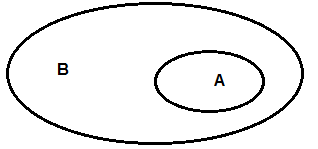
\includegraphics[width=\textwidth]{figures/KroegerIntroSemPragprepubv2g-img1.png}
\begin{tikzpicture}
 \node at (0,0) (A) {A}; 
 \node[left=3em of A] (B) {B};
 \node[fit =(A),draw,ellipse] (fit1) {};
 \node[fit =(B) (fit1),draw,ellipse] (fit2) {};
\end{tikzpicture}

  \textsf{A}\textbf{${\subseteq}$}\textsf{B}\\

\caption{\label{fig:key:1} Set inclusion (the subset \textbf{relation)}}
\end{figure}

\ea \label{ex:13.13}
\ea  \{a,b,c\} ${\subseteq}$ \{a,b,c,d,f\}\\
\ex \{a,b,c\} ${\not\subset}$ \{c,d,f\}  ** need correct symbol **\\
\ex \{a,b,c\} ${\subseteq}$ \{a,b,c\}\\
\ex ${\forall}$S (where S is a set), ∅ ${\subseteq}$ S
                       \z
\z


Every set is a subset of itself, because all the elements which are members of set A are by definition members of set A. For this reason, the proposition “A${\subseteq}$A” will be true whenever A is a well-defined set, as illustrated in (\ref{ex:13.13}c). If we want to specify that set A is a subset of set B, but that the two sets are not equal, we can write “A${\subset}$B”. This symbol means that set A is a \textsc{proper subset} of set B. The proposition “A${\subset}$A” will be false for any set A.



Since the elements of every set must be members of the current universal set U, “A${\subseteq}$U” must always be true. If “U${\subseteq}$A” is true, than it must be the case that A=U.



The \textsc{intersection} of two sets, written “A${\cap}$B”, is defined as the set consisting of all elements which are both members of A and members of B. We can illustrate this situation using the sets defined in \REF{ex:13.14}. By comparing the elements in set A with those in set B, we see that the two sets share only the following elements in common: 3, 4, and 6; so A${\cap}$B = \{3,4,6\}.


\ea \label{ex:13.14}
U = \{1,2,3,4,5,6,7,8,9,10\}\\
A = \{2,3,4,6\}\\
B = \{3,4,5,6,7,8\}
\z


\figref{fig:key:2} illustrates set intersection in the form of a diagram: the ovals represent two sets, labeled A and B, while the shaded portion which is included in both ovals represents the intersection of the two sets (A${\cap}$B). Another example in standard set notation is provided in \REF{ex:13.15}.

%\todo{drawobject}
\begin{figure}
\begin{tikzpicture}
\scope % A \cap B
\clip (0,0) circle (1);
\fill[fill=gray!40] (1,0) circle (1);
\endscope
\draw (0,0) circle (1)
      (1,0) circle (1);
\node at (-.5,0) {A};
\node at (1.5,0) {B};
\node at (0.5,-1.5) (text) {\textsf{A${\cap}$B}};
\draw[-{Triangle[]}] (text.north) -- (0.5,0);
\end{tikzpicture}
 
% % 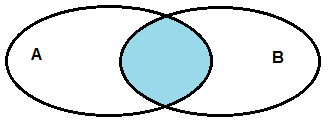
\includegraphics[width=\textwidth]{figures/KroegerIntroSemPragprepubv2g-img2.png}


\caption{\label{fig:key:2}: Set intersection}
\end{figure}

\ea \label{ex:13.15}
\{a,b,c\} ${\cap}$ \{c,d,f\} = \{c\}
\z


The \textsc{union} of two sets, written “A${\cup}$B”, is the set consisting of all elements which are either members of A or members of B. Returning to the sets defined in \REF{ex:13.14}, the union of the two sets is formed by combining all the elements from both, which yields the following result: A${\cup}$B = \{2,3,4,5,6,7,8\}. \figref{fig:key:3} illustrates this in the form of a diagram, and another example in standard set notation is provided in \REF{ex:13.16}.


\begin{figure}
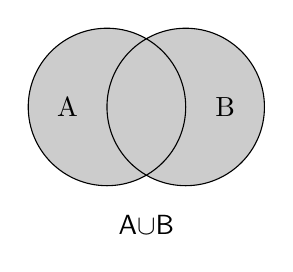
\begin{tikzpicture}
\scope % A \cap B
\clip (0,0) circle (1);
\fill[fill=gray!40] (1,0) circle (1);
\endscope
\draw[fill=gray!40] (0,0) circle (1)
      (1,0) circle (1);
\node at (-.5,0) {A};
\node at (1.5,0) {B};
\node at (0.5,-1.5) (text) {\textsf{A${\cup}$B}};
\end{tikzpicture}

\caption{\label{fig:key:3}Set union}
\end{figure}

\begin{stylepoints} \label{ex:13.16}
\{a,b,c\} ${\cup}$ \{c,d,f\} = \{a,b,c,d,f\}
\end{stylepoints}


The \textsc{complement} of set A, written as \=A or Aʹ, is defined as the set which contains all the elements of U that are not elements of A. Some simple examples are shown in \REF{ex:13.17}. Here, the only elements of U which are not in A are 1 and 5, so \=A = \{1,5\}. Similarly, the elements of U which are not in B are 1, 2, 5, and 6; so \=B = \{1,2,5,6\}.


\ea \label{ex:13.17}
U = \{1,2,3,4,5,6\}\\
A = \{2,3,4,6\}\\
\=A = \{1,5\}\\
B = \{3,4\}\\
\=B = \{1,2,5,6\}
\z


This basic notion of complement set involves complements relative to the universal set U. It is often useful to refer to the complement of one set relative to some other set. The complement of A relative to B, written “B–A”, is the set consisting of all elements which are members of B but not members of A.\footnote{This operation is sometimes referred to as “set subtraction.”} Another way of expressing this definition is the following: B–A = B${\cap}$\=A. \figref{fig:key:4} illustrates this in the form of a diagram, and several examples in standard set notation are provided in \REF{ex:13.18}.

%\todo{drawobject}
\begin{figure}
% [Warning: Draw object ignored]\\
\begin{tikzpicture}
\scope
\clip (-2,-2) rectangle (2,2)
      (1,0) circle (1);
\fill[white] (0,0) circle (1);
\endscope
\scope
\clip (-2,-2) rectangle (2,2)
      (0,0) circle (1);
\fill[gray!40] (1,0) circle (1);
\endscope
\draw (0,0) circle (1)
      (1,0) circle (1);
\node at (-.5,0) {A};
\node at (1.5,0) {B};
\node at (1.25,-1.5) (text) {\textsf{B–A}};
\draw[-{Triangle[]}] (text.north) -- (1.25,-.5);
\end{tikzpicture}
\caption{\label{fig:key:4} Set complementation}
\end{figure}

\begin{stylepoints} \label{ex:13.18}
\{a,b,c\} – \{b,c\} = \{a\}\\
\{a,b,c,d,f\} – \{a,b,c,j,k,p\} = \{d,f\}\\
A – ∅ = A\\
∅ – A = ∅\\
U – A = \=A
\end{stylepoints}


To summarize, we have defined three basic operations on sets (\textsc{intersection}, \textsc{union}, and \textsc{complement} or “difference”), and one relation between sets, namely \textsc{inclusion} (the \textsc{subset} relation). The three operations provide ways of combining two existing sets to define a new set. It is important to note that “A${\cap}$B”, “A${\cup}$B”, and “B–A” are names of sets; but “A${\subseteq}$B” is a proposition, a claim about the membership of the two sets, which could be true or false.



More precise definitions of set intersection, union, complementation, and inclusion (the subset relation) are provided in \REF{ex:13.19}. These definitions will help us to understand, for example, why the interpretation of an “and” statement frequently involves the intersection of two sets while the interpretation of an “or” statement frequently involves the union of two sets.


\ea \label{ex:13.19}
${\forall}$x [x ${\in}$ (A${\cap}$B)  $\leftrightarrow $  ((x${\in}$A) $\wedge$ (x${\in}$B))] \hfill [\textsc{intersection}]\\
${\forall}$x [x ${\in}$ (A${\cup}$B)  $\leftrightarrow $  ((x${\in}$A) $\vee$ (x${\in}$B))] \hfill [\textsc{union}]\\
${\forall}$x [x ${\in}$ (A–B)  $\leftrightarrow $  ((x${\in}$A) $\wedge$ (x${\notin}$B))] \hfill [\textsc{complement}]\\
(A ${\subseteq}$ B)  $\leftrightarrow $  ${\forall}$x [(x${\in}$A) → (x${\in}$B)] \hfill [\textsc{subset}]
\z

\section{Truth relative to a “model”}\label{sec:13.4}

We have noted several times that denotations, including the denotations of referring expressions and truth values of sentences, can only be evaluated relative to a particular situation of use. In order to develop and test a set of interpretive rules, which can correctly predict the denotation of a particular expression in any given situation, it is important to provide very explicit descriptions for the test situations. As stated above, this kind of description of a situation is called a \textsc{model}, and must include two types of information: (i) the \textsc{domain}, i.e., the set of all individual entities in the situation; and (ii) the denotation sets for the basic vocabulary items in the expressions being analyzed.



As a first illustration of how the system works, let us return to our simple situation containing just three individuals: King Henry VIII, Anne Boleyn, and Thomas More. Our model of this situation, which we might call Model 1, would provide the information listed in \REF{ex:13.20}. We often use the name “U” as a convenient way to refer to the domain (the “universal set” of individuals). The notation \textsc{$\llbracket$x}$\rrbracket$  represents the denotation (or “semantic value”) of x within the current model. This notation can be used either for object language expressions or for logical formulae; so, for example, $\llbracket$SNORE$\rrbracket$  names the same set as $\llbracket$\textit{snores}$\rrbracket$ . By convention we use small letters for logical “constants”, e.g. proper names, and capital letters for predicates.


\ea \label{ex:13.20}Model 1\\
\begin{enumerate}[label=\roman*.]
\item the set of individuals U = \{ King Henry VIII, Anne Boleyn, Thomas More \}
\item denotations\textsc{:\\
{}$\llbracket$}\textsc{MAN}$\rrbracket$  = \{ King Henry VIII, Thomas More \}\\
\textsc{$\llbracket$}WOMAN$\rrbracket$  = \{ Anne Boleyn \}\\
\textsc{$\llbracket$}SNORE$\rrbracket$  = \{ King Henry VIII \}\\
\textsc{$\llbracket$}a$\rrbracket$  = Anne Boleyn\\
\textsc{$\llbracket$}h$\rrbracket$  = King Henry VIII\\
\textsc{$\llbracket$}t$\rrbracket$  = Thomas More
\end{enumerate}
\z

The denotation sets encode information about the current state of the world. For example, this model indicates that King Henry VIII is the only person in the current situation who snores. We can use the defined vocabulary items to build simple declarative sentences about the individuals in this situation, and then try to provide interpretations for each sentence in terms of set membership, as illustrated in \REF{ex:13.21}. These interpretations express the truth conditions for each sentence. We can use them to evaluate the truth of each sentence relative to Model 1. For example, the sentence in (\ref{ex:13.21}a), \textit{Thomas More is a man}, will be true in any situation where the individual Thomas More is a member of the denotation set of the word \textit{man}. Since this is the case in Model 1, the sentence is true relative to this model.



\eabox{ \label{ex:13.21}
\fittable{
\begin{tabular}{llllll}
% \lsptoprule

\bfseries\scshape ~~~English sentence & \multicolumn{2}{l}{\bfseries\scshape logical form} & \multicolumn{2}{l}{\bfseries\scshape interpretation} & \bfseries\scshape truth value\\
% \midrule

a. \textit{Thomas More is a man}. & \multicolumn{2}{l}{MAN(t)
\newline
Thomas More ${\in}$ \textsc{$\llbracket$}MAN$\rrbracket$ } & \multicolumn{2}{l}{ T} & \\

b. \textit{Anne Boleyn is} \textit{a man or} \textit{a woman}. & \multicolumn{2}{l}{MAN(a) $\vee$ WOMAN(a)} & \multicolumn{2}{l}{Anne Boleyn ${\in}$
\newline
(\textsc{$\llbracket$}MAN$\rrbracket$  ${\cup}$ \textsc{$\llbracket$}WOMAN$\rrbracket$ )} & T\\

c. \textit{Henry VIII is a man who snores}. & \multicolumn{2}{l}{MAN(h) $\wedge$ \textsc{SNORE}(h)} & \multicolumn{2}{l}{Henry VIII ${\in}$ (\textsc{$\llbracket$}MAN$\rrbracket$  ${\cap}$ \textsc{$\llbracket$SNORE}$\rrbracket$ )} & T\\
\biberror{sth missing}&
 \textsc{$\llbracket$WO}MAN$\rrbracket$  ${\cap}$ \textsc{$\llbracket$SNORE}$\rrbracket$  = ∅Td.\\ \textit{All men snore}.& \multicolumn{2}{l}{${\forall}$x[MAN(x) → \textsc{SNORE}(x)]} & \multicolumn{2}{l}{\textsc{$\llbracket$}MAN$\rrbracket$  ${\subseteq}$ \textsc{$\llbracket$SNORE}$\rrbracket$ } & F\\
 
\multicolumn{1}{l}{¬${\exists}$x[WOMAN(x) $\wedge$ \textsc{SNORE}(x)]
\newline
d. \textit{No women snore.}} &  & \multicolumn{2}{l}{} & \multicolumn{2}{l}{}\\
% \lspbottomrule
\end{tabular}
}
}
\todo{check alphabetical labels}

The interpretations in (\ref{ex:13.21}b--e) can be derived from the corresponding logical forms, based on the definitions of intersection, union, and subset provided in \REF{ex:13.}. For example, the \textit{or} statement in (\ref{ex:13.19}b) constitutes a claim that a certain individual (Anne Boleyn) is a member of the union of two sets, because the definition of A${\cup}$B involves an \textit{or} statement. Once the truth conditions are stated in terms of set relations, we can determine the truth values for each sentence by inspecting the membership of the denotation sets specified in the model. The statement in (\ref{ex:13.21}b) is true relative to Model 1 because the individual Anne Boleyn is a member of the set $\llbracket$WOMAN$\rrbracket$ , and thus a member of $\llbracket$MAN$\rrbracket$  ${\cup}$ $\llbracket$WOMAN$\rrbracket$ .


\section{Rules of interpretation}\label{sec:13.5}

Stating the truth conditions for individual sentences like those in \REF{ex:13.21} is a useful first step, but does not yet replicate what speakers can do in their productive use of the language. Ultimately our goal is to provide general rules of interpretation which will predict the correct truth conditions for sentences based on their syntactic structure. As a further step toward this goal, let us return to the sentence in (\ref{ex:13.22}a), which we have already discussed several times.


\ea \label{ex:13.22}
\ea \textit{King Henry VIII snores}.\\
\ex \textit{Anne Boleyn} \textit{snores}.
                       \z
\z


We have already stated an informal rule of interpretation for simple sentences: the proposition expressed by a (declarative) sentence will be true just in case the referent of the subject NP is a member of the denotation set of the VP. We can now restate this rule in a slightly more formal manner. We will assume that the basic syntactic structure of the clause is [NP VP]. The semantic rule we wish to state operates in parallel with the syntactic rule which licenses this structure, as suggested in \REF{ex:13.23}. (Recall that the semantic value, i.e. the denotation, of a sentence is its truth value.)


\ea \label{ex:13.23}
\textbf{syntax}: S  →  NP\textsubscript{subj}  VP\\
\textbf{semantics}: The semantic value of a sentence is “true” if the semantic value of the subject is a member of the set which is the semantic value of the VP, and “false” otherwise;\\
{}$\llbracket$S$\rrbracket$  = ‘true’  iff  $\llbracket$NP\textsubscript{subj}$\rrbracket$  ${\in}$ $\llbracket$VP$\rrbracket$ 
\z


Applying this rule to the sentence in (\ref{ex:13.22}a), we get the formula in \REF{ex:13.24}. This formula says that the sentence will be true just in case King Henry VIII is a member of the denotation set of \textit{snores}. Since this is true in our model, the sentence is true relative to this model. The same rule of interpretation allows us to determine that sentence (\ref{ex:13.22}b) is false relative to this model.


\ea \label{ex:13.24}
{}$\llbracket$\textit{King Henry VIII snores}$\rrbracket$  = ‘true’  iff  $\llbracket$\textit{King Henry VIII}$\rrbracket$  ${\in}$ $\llbracket$\textit{snores}$\rrbracket$ 
\z


The statement in \REF{ex:13.24} can be expressed in logical notation as in (\ref{ex:13.25}a). This formula is a specific instance of the general rule for evaluating the truth of propositions involving a one-place predicate. This general rule, shown in (\ref{ex:13.25}b), states that the proposition \textit{P(α)} is true if and only if the entity denoted by \textit{α} is an element of the denotation set of \textit{P}.

\ea \label{ex:13.25}
\ea  $\llbracket$SNORE(h)$\rrbracket$  = ‘true’  iff  $\llbracket$h$\rrbracket$  ${\in}$ $\llbracket$SNORE$\rrbracket$ 
\ex  if α refers to an entity and P is a one-place predicate,\\
  then  $\llbracket$P(α)$\rrbracket$  = ‘true’  iff  $\llbracket$α$\rrbracket$  ${\in}$ $\llbracket$P$\rrbracket$ 
\z \z


Let us now add a few more vocabulary items to our simple model, calling the new version Model 1ʹ. This revised model presumably reflects the early period of the marriage, ca. 1532--1533 AD, when Henry and Anne were happy and in love. Note also that Thomas More had fallen out of favor with the king around this time.


\ea \label{ex:13.26} Model 1ʹ\\
\begin{enumerate}[label=\roman*.]
\item the set of individuals U = \{ King Henry VIII, Anne Boleyn, Thomas More \}
\item denotations\textsc{:\\
{}$\llbracket$}\textsc{MAN}$\rrbracket$  = \{ King Henry VIII, Thomas More \}\\
\textsc{$\llbracket$}WOMAN$\rrbracket$  = \{ Anne Boleyn \}\\
\textsc{$\llbracket$}SNORE$\rrbracket$  = \{ King Henry VIII \}\\
\textsc{$\llbracket$}HAPPY$\rrbracket$  = \{ King Henry VIII, Anne Boleyn \}\\
\textsc{$\llbracket$}LOVE$\rrbracket$  = \{ $\langle$King Henry VIII, Anne Boleyn$\rangle$, $\langle$ Anne Boleyn, King Henry VIII$\rangle$ \}\\
\textsc{$\llbracket$}ANGRY\_AT$\rrbracket$  = \{ $\langle$King Henry VIII, Thomas More$\rangle$ \}\\
\textsc{$\llbracket$}a$\rrbracket$  = Anne Boleyn\\
\textsc{$\llbracket$}h$\rrbracket$  = King Henry VIII\\
\textsc{$\llbracket$}t$\rrbracket$  = Thomas More
\end{enumerate}
\z

Model 1ʹ includes some two-place (i.e, transitive) predicates, and should allow us to evaluate simple transitive sentences like those in \REF{ex:13.27}. The denotation set of a transitive predicate like LOVE or ANGRY\_AT is not a set of individuals, but a set of ordered pairs. Sentence (\ref{ex:13.27}a) expresses the proposition stated by the logical formula in (\ref{ex:13.28}a). The truth conditions for this proposition are stated in terms of set membership in (\ref{ex:13.28}b): the proposition will be true just in case the ordered pair $\langle$King Henry VIII, Anne Boleyn$\rangle$ is a member of the denotation set of LOVE. Since this is true in Model 1ʹ, sentence (\ref{ex:13.27}a) is true with respect to this model. The formula in (\ref{ex:13.28}b) is an instance of the general pattern stated in (\ref{ex:13.28}c).


\ea \label{ex:13.27}
\ea \textit{King Henry VIII loves Anne Boleyn}.\\
\ex \textit{King Henry VIII is angry at} \textit{Thomas More}.
                       \z
\z

\ea \label{ex:13.28}
\ea  LOVE(h,a)\\
\ex  $\llbracket$LOVE(h,a)$\rrbracket$  = ‘true’  iff  $\langle$$\llbracket$h$\rrbracket$ ,$\llbracket$a$\rrbracket$ $\rangle$ ${\in}$ $\llbracket$LOVE$\rrbracket$ 
\ex  if α, β refer to entities and P is a two-place predicate,\\
  then  $\llbracket$P(α,β)$\rrbracket$  = ‘true’  iff  $\langle$$\llbracket$α$\rrbracket$ ,$\llbracket$β$\rrbracket$ $\rangle$ ${\in}$ $\llbracket$P$\rrbracket$ 
\z \z


So far we have been dealing with the meanings of complete sentences all at once. This is possible only for the very simple kinds of sentences discussed thus far, but more importantly, it misses the point of the exercise. If we hope to account for the compositional nature of sentence meaning, modeling speakers’ and hearers’ ability to interpret novel sentences, we need to pay attention to syntactic structure. The sentences in \REF{ex:13.27} share the same basic syntactic structure as those in \REF{ex:13.22}, namely [NP VP]. This suggests that the rule of interpretation stated in \REF{ex:13.23} should apply to the sentences in \REF{ex:13.27} as well.



The main syntactic difference between the sentences in \REF{ex:13.27} and those in \REF{ex:13.22} is the structure of VP: transitive in \REF{ex:13.27}, intransitive in \REF{ex:13.22}. In order to apply rule \REF{ex:13.23} to the sentences in \REF{ex:13.27}, we need another rule which will provide the semantic value of a transitive VP. Intuitively, rule \REF{ex:13.23} says that the proposition expressed by a (declarative) sentence will be true just in case the referent of the subject NP is a member of the denotation set of the VP. So we need to say that sentence (\ref{ex:13.27}a) will be true just in case King Henry VIII belongs to a certain set. What is the relevant set? It would be the set of all individuals that love Anne Boleyn. This set will be the denotation set of the VP \textit{loves Anne Boleyn}. The standard notation for defining such a set is shown in (\ref{ex:13.29}a), which says that the denotation set of this VP will be the set of all individuals x such that the ordered pair $\langle$x, Anne Boleyn$\rangle$ is an element of the denotation set of the transitive verb \textit{love}.


\ea \label{ex:13.29}
\ea $\llbracket$\textit{loves Anne Boleyn}$\rrbracket$  = \{x: $\langle$x, Anne Boleyn$\rangle$ ${\in}$ $\llbracket$LOVE$\rrbracket$ \}
\ex \textbf{syntax}: VP  →  V\textsubscript{trans}  NP\textsubscript{obj}\\
\textbf{semantics}: The semantic value of a VP containing a transitive verb meaning P together with an object NP meaning α is the set of all individuals x for which P(x,α) is true;\\
{}$\llbracket$VP$\rrbracket$  =  \{x: $\langle$x, $\llbracket$NP\textsubscript{obj}$\rrbracket$ $\rangle$ ${\in}$ $\llbracket$V\textsubscript{trans}$\rrbracket$ \}
\z \z


The general rule for deriving denotation sets of transitive VPs is stated in (\ref{ex:13.29}b). The denotation sets formed by this rule are sets of individuals, so it makes sense to ask whether the referent of a subject NP is a member of one of these denotation sets. In other words, the denotation sets formed by rule (\ref{ex:13.29}b) are the right kind of sets to function as VP denotations in rule \REF{ex:13.23}. So this approach allows us to model the step-wise derivation of sentence denotations. The rule of interpretation stated in \REF{ex:13.23} applies to both transitive and intransitive sentences. In the case of transitive sentences, rule (\ref{ex:13.29}b) “feeds”, or provides the input to, rule \REF{ex:13.23}.



Rule \REF{ex:13.23} can also be applied to intransitive sentences with non-verbal predicates like those in \REF{ex:13.30}, provided we can determine the denotation set of the VP.


\ea \label{ex:13.30}
\ea \textit{King Henry VIII is happy}.\\
\ex \textit{King Henry VIII is a man}.\\
\ex \textit{King Henry VIII is a happy man}.
                       \z
\z


We can assume that the semantic contribution of the copular verb \textit{is} is essentially nil (apart from tense, which we are ignoring for the moment). That means that the denotation set of the VP \textit{is happy} will be identical to $\llbracket$HAPPY$\rrbracket$ , which is a set of individuals. For now we will also assume that the semantic contribution of the indefinite article in a predicate NP is nil.\footnote{This assumption applies only to predicate NPs, and not to indefinite NPs in argument positions.} So the denotation set of the VP \textit{is a man} will be identical to $\llbracket$MAN$\rrbracket$ , which is also a set of individuals. In general, the denotation sets of common nouns and many adjectives are of the same type as the denotation sets of intransitive verbs; this is observable in the denotations assigned in \REF{ex:13.26}. So no extra work is needed to interpret sentences (\ref{ex:13.30}a--b), using rule \REF{ex:13.23}.



Sentence (\ref{ex:13.30}c) is more complex, because the predicate NP contains a modifying adjective as well as the head noun. As with transitive verbs, we can determine the denotation set of the VP (in this case, \textit{is a happy man}) by asking what set the sentence asserts that Henry VIII belongs to? Here the relevant set is the set of happy men, i.e., the set of all individuals who are both happy and men.



The combination of word meanings in \textit{happy man} follows the same pattern we have already discussed in connection with the phrase \textit{yellow submarine}. The proposition asserted in (\ref{ex:13.30}c) might be represented by the formula in (\ref{ex:13.31}a). The truth conditions for this proposition are stated in terms of set membership in (\ref{ex:13.31}b). (Recall the definition of intersection given in \REF{ex:13.19}.) The general rule for interpreting modifying adjectives is stated in (\ref{ex:13.31}c); we use the category label Nʹ for the constituent formed by A+N. Ignoring once again any possible semantic contribution of the copula and the indefinite article, the denotation set of the VP \textit{is a happy man} is simply $\llbracket$HAPPY$\rrbracket$  ${\cap}$ $\llbracket$MAN$\rrbracket$ . This is a set of individuals, and so rule \REF{ex:13.23} will apply correctly to sentence (\ref{ex:13.30}c) as well.


\ea \label{ex:13.31}
\ea  HAPPY(h) $\wedge$ MAN(h)\\
\ex  $\llbracket$HAPPY(h) $\wedge$ MAN(h)$\rrbracket$  = ‘true’  iff  $\llbracket$h$\rrbracket$  ${\in}$ ($\llbracket$HAPPY$\rrbracket$  ${\cap}$ $\llbracket$MAN$\rrbracket$ )
\ex  \textbf{syntax}: Nʹ  →  A N\\
\textbf{semantics}: The semantic value of an Nʹ constituent containing a modifying adjective and a head noun is the intersection of the semantic values of the adjective and noun;\\
{}$\llbracket$A N$\rrbracket$  =  $\llbracket$A$\rrbracket$  ${\cap}$ $\llbracket$N$\rrbracket$ 
\z \z

\section{Conclusion}\label{sec:13.6}

In this chapter we have worked through a compositional analysis for the meanings of simple sentences like those in \REF{ex:13.4}, \REF{ex:13.27}, and \REF{ex:13.30}. We have developed a rule of semantic interpretation for simple clauses of the form [NP VP] (see rule ), a similar rule for transitive VPs (rule b), and a rule for adjective modifiers (\ref{ex:13.31}c). We have shown how these rules can be applied in a step-wise fashion to derive the truth-conditions of a simple sentence from the denotations of the words that it contains and the manner in which those words are combined syntactically.



In discussing the meanings of quantifiers, conditionals, tense markers etc. in later chapters we will focus more on understanding the phenomena than on formalizing the rule system, but we will still draw heavily on the concepts introduced in this chapter. Moreover, an important assumption in everything that follows is that our description of the meanings of these elements must be compatible with the kind of compositional analysis illustrated in this chapter.



\furtherreading



Good brief introductions to set theory are provided in \citet[ch. 2]{AllwoodEtAl1977},
\citet[ch. 2]{Martin1987},
\citet[ch. 2]{Coppock2016}; and 
\citet[ch. 5]{McCawley1981a}. Readable introductory textbooks include \citet{Halmos1960} and \citet{Enderton1977}. Formal introductions to truth-conditional semantics are provided in  \citet{DowtyEtAl1981} and \citet{HeimKratzer1998}. An informal discussion of this approach is presented in \citet{Bach1989}. A brief introduction to Model Theory is provided by \citet{Hodges2013}. Standard textbooks for this topic include \citet{ChangKeisler1990} and \citet{Hodges1997}.


\subsection*{Discussion exercises}
\paragraph*{A. Set theory}

Fill in the following tables:

\eabox{ \label{ex:13.}%1
    \label{ex:key:1} 
\begin{tabularx}{\textwidth}{lQQQ}
\lsptoprule
 & Set A & Set B & A${\cap}$B  \\
\midrule
a. &  the set of all mammals & the set of all animals that lay eggs & the set of all \textsc{monotremes} (Platypus plus four species of echidna)\\
\tablevspace
b. &  \{p,q,s,t\} & \{q,t,w,x\} & \\
\tablevspace
c. &  the set of all odd numbers & the set of all even numbers & \\
\tablevspace
d. &  the set of all Hollywood stars & \biberror{people with 2-syllable first names}\\
\tablevspace
e. & the set containing all members of the Beatles & the set of all governors of California (past and present) & \\
\lspbottomrule
\end{tabularx}
}
 
\eabox{ \label{ex:13.}%2
    \label{ex:key:2}
\begin{tabularx}{\textwidth}{lQQQ}
\lsptoprule
 &Set A & Set B & A${\cup}$B\\
 \midrule
a. & the set of all the books of the Old Testament & the set of all the books of the New Testament & the set of the canonical books of the Bible  \\
\tablevspace
b. & \{p,q,s,t\} & \{q,t,w,x\} & \\
\tablevspace
c. & the set of all odd numbers & the set of all even numbers & \\
\tablevspace
d. & the set of all members of the  British House of Lords & the set of all members of the British House of Commons & \\
\tablevspace
e. & the set of all female     British monarchs            & the set of all female French monarchs\footnote{Note: there were no female French monarchs.} & \\
\lspbottomrule
\end{tabularx} 
    }
    
\eabox{ \label{ex:13.}%3
    \label{ex:key:3}
    
\begin{tabularx}{\textwidth}{lQQQ}
\lsptoprule
 Set A & Set B & A–B\\
 \midrule
a. & nations that have won at least one FIFA World Cup title & nations that have won a FIFA World Cup title playing in their own homeland
& \{Brazil, Spain\} (as of Dec. 2016) \\
\tablevspace
b. & \{p,q,s,t\} & \{q,t,w,x\} & \\
\tablevspace
c. & the set of all integers & the set of all even numbers & \\
\tablevspace
d. & the set of all cordates & the set of all renates & \\
\tablevspace
e. & the set of all French monarchs & the set of all female French monarchs & \\
\lspbottomrule
\end{tabularx}
    }
    
\todo{check labels}    
\eabox{ \label{ex:13.}%4
    \label{ex:key:4}
\begin{tabularx}{\textwidth}{lQQQ}
\lsptoprule
& YesSet A & Set B & A${\subseteq}$B?\\
\midrule
\biberror{ex} \{p,q,s,t\} & \{q,t,w,x\} & \\
a. & the set of all mammals & the set of all \textsc{monotremes} & \\
\tablevspace
b. & the set of all odd numbers & the set of all integers & \\
\tablevspace
c. & the set of all cordates & the set of all renates & \\
\tablevspace
d. & the set of all Indo-European  languages & the set of all SVO languages & \\
\lspbottomrule
\end{tabularx}
    }
\paragraph*{B. Model theory}

\ea \label{ex:13.}%1
    \label{ex:key:1} 
         Sketch a picture of the situation defined by the following model:

    \z
\begin{enumerate}
\item the set of individuals U = \{Able, Baker, Charlie, Doug, Echo, Fred, Geronimo\}
\item denotation assignments\textsc{:\\
{}$\llbracket$}\textsc{FISH}$\rrbracket$  = \{Able, Baker, Charlie, Doug\}\\
\textsc{$\llbracket$}SUBMARINE$\rrbracket$  = \{Echo\}\\
\textsc{$\llbracket$}SEAHORSE$\rrbracket$  = \{Fred, Geronimo\}\\
\textsc{$\llbracket$}RED$\rrbracket$  = \{Able, Baker, Fred\}\\
\textsc{$\llbracket$}GREEN$\rrbracket$  = \{Charlie, Geronimo\}\\
\textsc{$\llbracket$}BLUE$\rrbracket$  = \{Doug, Echo\}\\
\textsc{$\llbracket$}SWIM$\rrbracket$  = \{Able, Baker, Charlie, Doug, Fred, Geronimo\}\\
\textsc{$\llbracket$}OCTOPUS$\rrbracket$  = ∅\\
{}$\llbracket$FOLLOW$\rrbracket$  = \{$\langle$Able, Echo$\rangle$, $\langle$Doug, Able$\rangle$, $\langle$Doug, Echo$\rangle$, $\langle$Charlie, Fred$\rangle$\}\\
\textsc{$\llbracket$}a$\rrbracket$  = Able  \textsc{$\llbracket$}e$\rrbracket$  = Echo\\
\textsc{$\llbracket$}b$\rrbracket$  = Baker  \textsc{$\llbracket$}f$\rrbracket$  = Fred\\
\textsc{$\llbracket$}c$\rrbracket$  = Charlie  \textsc{$\llbracket$}g$\rrbracket$  = Geronimo\\
\textsc{$\llbracket$}d$\rrbracket$  = Doug
\end{enumerate}

\ea \label{ex:13.}%2
    \label{ex:key:2} 
          Complete the following table by providing logical formulae and set-theoretic interpretations for sentences (e–i), and evaluate the truth value of each sentence relative to the model provided above.
    \z 

\begin{tabularx}{\textwidth}{lQQQQ}
\lsptoprule
& \bfseries\scshape English sentence & \bfseries\scshape logical form & \bfseries\scshape set interpretation & \textbf{\textsc{current truth value}}\\
\midrule
a. & \textit{Geronimo is a seahorse}. & SEAHORSE(g) & Geronimo ${\in}$ \textsc{$\llbracket$}SEAHORSE$\rrbracket$  & T\\
b. & \textit{Doug is a blue fish}.

BLUE(d) $\wedge$ \textsc{FISH}(d) & Doug ${\in}$ (\textsc{$\llbracket$}BLUE$\rrbracket$  ${\cap}$ \textsc{$\llbracket$FISH}$\rrbracket$ ) & T & \\
c. & \textit{Charlie is red or green}. & RED(c) $\vee$ GREEN(c) & Charlie ${\in}$ (\textsc{$\llbracket$}RED$\rrbracket$  ${\cup}$ \textsc{$\llbracket$}GREEN$\rrbracket$ ) & T\\
d. & \textit{All fish are red}. & ${\forall}$x[\textsc{FISH}(x) → RED(x)] & \textsc{$\llbracket$FISH}$\rrbracket$  ${\subseteq}$ \textsc{$\llbracket$}RED$\rrbracket$  & F\\
e. & \textit{Echo swims}. &  &  & \\
f. & \textit{All fish swim}. &  &  & \\
g. & \textit{No submarine is red}. &  &  & \\
h. & \textit{Two fish are red}. &  &  & \\
i. & \textit{Some seahorse is green}. &  &  & \\
\lspbottomrule
\end{tabularx}
\todo{check alphabetical labels}

\ea \label{ex:13.}%3
    \label{ex:key:3}
    Draw annotated tree diagrams for the following sentences showing how their truth conditions would be derived compositionally from our rules of interpretation:\\
\ea \label{ex:13.} \textit{Henry snores}.\\
\ex \textit{Henry loves Jane}.\\
\ex \textit{Henry is a happy man}.
                       \z
    \z

\subsection*{Homework exercises}
\begin{stylepoints}
\textbf{A:} Assume that the following individuals are included in our universe of discourse:\\
{}$\llbracket$b$\rrbracket$  = Mrs. Bennet\\
{}$\llbracket$c$\rrbracket$  = Mr. Collins\\
{}$\llbracket$d$\rrbracket$  = Mr. Darcy\\
{}$\llbracket$e$\rrbracket$  = Elizabeth (Bennet)\\
{}$\llbracket$l$\rrbracket$  = Lydia (Bennet)\\
{}$\llbracket$w$\rrbracket$  = Mr. Wickham
\end{stylepoints}

\begin{stylepoints}
(i) For each of the following logical formulae, provide an English translation and an interpretation stated in terms of set notation.\\
(ii) Create a model under which sentences (\ref{ex:13.}b--c) will be false, and the rest (including (\ref{ex:13.}a)) will be true.\footnote{Patterned loosely after \citet[350]{Saeed2009}.}
\end{stylepoints}

\paragraph*{Example:}
\begin{enumerate}
\item LOVE(d,e)
\end{enumerate}

\textsf{[Model answer]:\\
English translation: ‘Mr. Darcy loves/loved Elizabeth.’\\
truth conditions:} $\langle$\textsf{Darcy, Elizabeth}$\rangle$\textsf{} ${\in}$\textsf{} $\llbracket$\textsf{LOVE}$\rrbracket$ 

\begin{enumerate}
\item REJECT(e,c)
\item ${\forall}$x [(MAN(x) $\wedge$ WEALTHY(x)) → ADMIRE(b,x)]
\item ${\exists}$x [MAN(x) $\wedge$ WEALTHY(x) $\wedge$ ADMIRE(b,x)]
\item ¬${\exists}$x [WOMAN(x) $\wedge$ LOVE(x,c)]
\item DECEIVE(w,l) $\wedge$ RESCUE(d,l)
\item ${\forall}$x [WOMAN(x) → CHARM(w,x)] $\wedge$ ${\forall}$y [MAN(y) → ANGER(w,y)]
\end{enumerate}

